\section{Datenbank}

Die Anforderungen der App an die Datenbank sind einfach und leicht überschaubar.

\subsection{Übersicht Datenbankfelder der Items}
\label{sec:Felder}

In der Tabelle \ref{tab:Datenbankfelder}  sind die Datenbankfelder für jedes Medium, Bücher, Filme und Spiele aufgeführt.

\begin{table} [htbp]
	\begin{center}
		\begin{tabular}{|l|l|l|l|}
			\rowcolor{black} {\color{white}\textbf{Allgemein}} & {\color{white}\textbf{Bücher}} & {\color{white}\textbf{Filme}} & {\color{white}\textbf{Spiele}} \\
			Barcode & Verlag & Studio & Entwickler\\ \hline
			\rowcolor{DarkSeaGreen} Titel & Auflage & Speichermedium & System \\ \hline			Medientyp & Autor& Regisseur & FSK \\ \hline
			\rowcolor{DarkSeaGreen} Genre & & FSK & \\ \hline
			Sprache & & Länge & \\ \hline
			\rowcolor{DarkSeaGreen} Erscheinungsjahr & & & \\ \hline
			Bewertung & & & \\ \hline
			\rowcolor{DarkSeaGreen} Lagerplatz & & & \\ \hline
			Verleihstatus & & & \\ \hline
			\rowcolor{DarkSeaGreen} Bemerkung & & & \\ \hline		
		\end{tabular}
	\caption{Datenbankfelder}
	\label{tab:Datenbankfelder}
	\end{center}
\end{table}

\newpage

\begin{landscape}
	\section{Übersicht Datenbank}
	\label{sec:UebersichtDB}
	\begin{figure}[htbp]
		\centering
		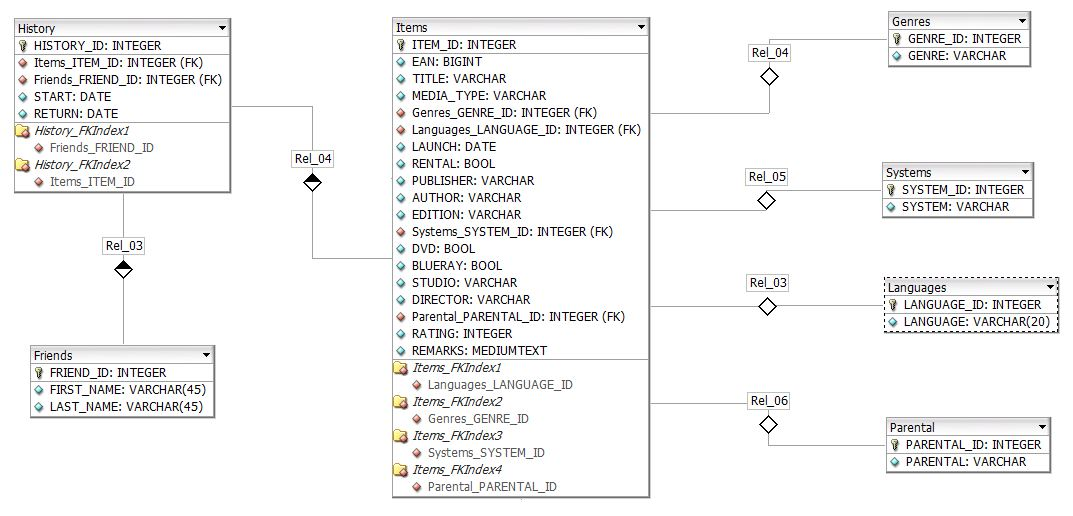
\includegraphics[scale=0.75]{pic/DbDesign}
		\caption{Überblick Datenbank}
	\end{figure}
\end{landscape}